%\newpage
%\subsection{Dataset}

Next, we apply our method to brain imaging data from the anonymized multimodal
neuroimaging ``Mother Of all Unification Studies'' (MOUS) dataset
\citep{schoffelen2019204}. The dataset contains magneto-encephalography (MEG)
recordings of 102 healthy native-Dutch adults who participated in a reading
task.
%
Subjects were exposed to a rapid serial visual presentation of Dutch words. The
word lists consisted of 120 sentences, and scrambled lists of the same words.
Each word was presented on the computer screen for 351ms on average (min: 300ms,
max: 1400ms). Successive words were separated by a blank screen for 300ms, and
successive sentences were separated by an empty screen for a few (3-4) seconds.

\subsubsection{MEG preprocessing}

The raw MEG data was bandpass-filtered between 0.1 and 40Hz using MNE-Python
default parameters \citep{gramfort2013meg, gramfort2014mne}. Specifically, we used a zero-phase finite impulse
response filter (FIR) with a Hamming window and with transition bands of 0.1Hz
and 10Hz for the low and high cut-off frequencies.

The raw data was then segmented 100ms before word onset and 1s after
word onset ($t=0$ms corresponds to word onset). Finally, each resulting
segment was baseline-corrected between -100ms and 0ms, and decimated by 5 and
thus led a sampling frequency of 240Hz. Figure 1 in the supplementary material
shows the average response of the magnetometers evoked by the words presented
to the first subject.

For each subject and each time sample relative to word onset, we
build an observation matrix $Y \in \mathbb{R}^{n \times d_y}$ of $n\approx$ 2700 words
by $d_y=301$ MEG channels (273 magnetometers and 28 compensation channels). Each
of the columns of $Y$ is normalized to have zero mean and unit variance.

\subsubsection{Word features} We annotated each word with 38 features: 26
correspond to the count of each letter in the word (from 'a' to 'z',
independently of their case), the total number of letters ('word length'), the
frequency of the word in natural language (using the Zipf logarithmic scale
of \citep{van2014subtlex}), and the part-of-speech tags (i.e. NOUN, PROPN (proper
noun), VERB, PRON (pronoun), CONJ (conjunction), DET (determinant), ADJ
(adjective), ADV (adverb), and NUM (numerical)) using Spacy \citep{spacy2} and
WordFreq \citep{speerwordfreq}. For clarity purposes, we refer to these
features using two broad categories: visual (i.e. each letter and the total
number of letters) and lexical (part-of-speech and word frequency). This
procedure yields an $X \in \mathbb{R}^{n \times d_x}$ matrix of $n\approx$ 2700 words by
$d_x=38$ features for each subject. Each of the columns of $X$ is normalized to
have a mean and a standard deviation of 0 and 1 respectively.

\subsubsection{Methods}

Our goal is to identify which word features ($X$) lead to a reliable modulation of brain activity as measured with MEG recordings ($Y$) at each time sample and for each subject separately. To this aim,
we compare three methods: forward regression, backward regression, and back-to-back regression.
Corresponding results can be found in Figure \ref{fig:meg_twocurves}.

\begin{figure}[t!]
  \centering
  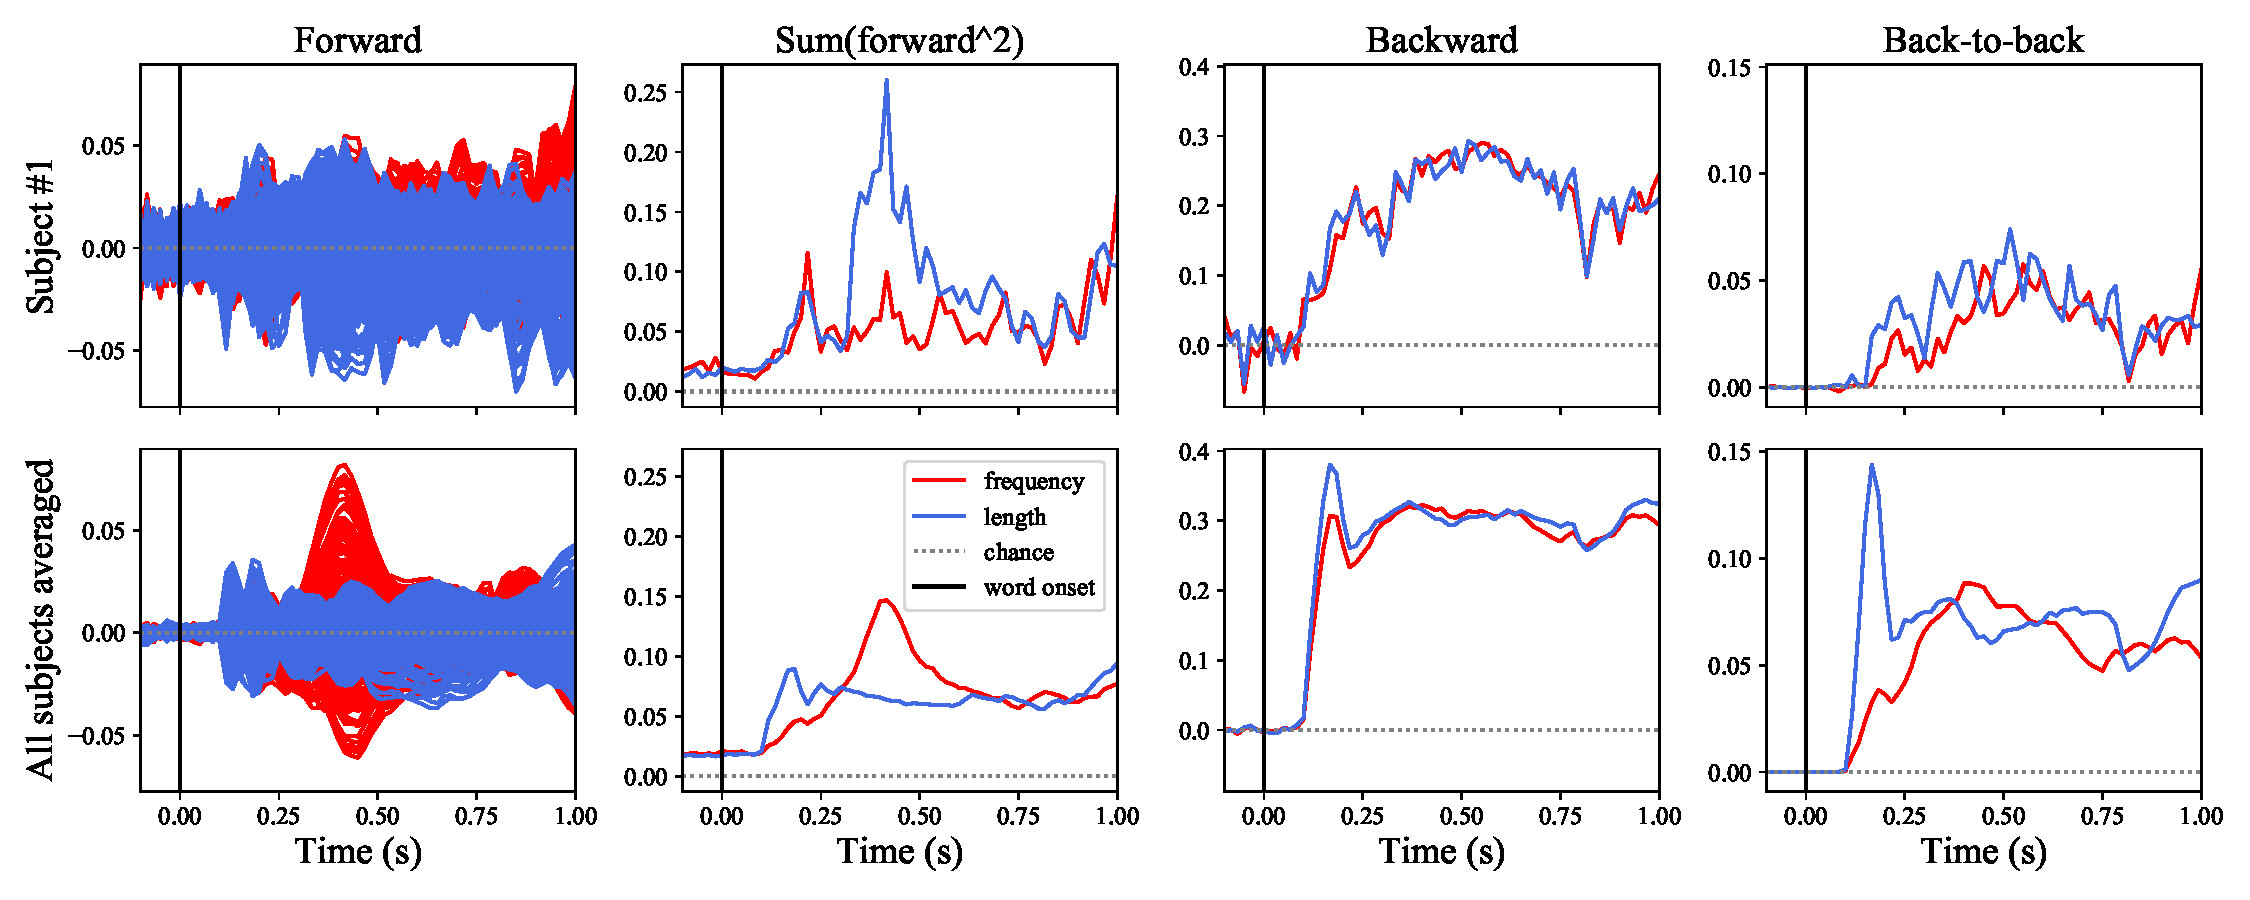
\includegraphics[width=\textwidth, trim=0cm 0cm 0cm 0cm, clip=True]{figures/meg_twocurves.pdf}
  \caption{We applied forward regression (a.k.a encoding coefficients), backward regression (a.k.a decoding scores) and B2B regression on 301-sensor MEG recordings of brain activity, while subjects were flashed with individual words every $\approx$650ms. Top row: the first subject. Bottom row: average across subjects. Each line represent the link between word features $X$ and MEG signals $Y$
  as a function of time relative to word onset ($x$ axis). The $y$-axis varies for each model (forward: H coefficients; backward: pearson correlation coefficients; B2B: $\hat E$). Forward regression makes prediction for each MEG channel independently; detecting an effect thus requires an additional average of the norm and can diminish sensitivity. Backward regression operates across all channels, but does not learn to disambiguate the two word features. B2B disambiguates these two factors consistently with previous neuroscientific work \cite{kutas2011thirty}\citep{pegado2014timing}
  showing early responses ($\approx$ 150ms) to word length and later responses
  ($\approx$ 400ms) to word frequency.}
  \label{fig:meg_twocurves}
\end{figure}

Forward regression was performed with an $\ell_2$-regularized least-squares regression $H \in \mathbb{R}^{d_x \times d_y}$ from $X$ to $Y$, and estimates the causal influence $E_{i,i}$ as $\| H_{i, :} \|^2$.
%
Backward regression was performed with an $\ell_2$-regularized least-squares regression $G \in \mathbb{R}^{d_y \times d_x}$ from $Y$ to $X$, and estimates the causal influence $E_{i, i}$ as the Pearson correlation between the $i$-th column of $X$ and the $i$-th column of $YG$, using a validation sample.
%
Finally, we used the back-to-back regression was performed using two $\ell_2$-regularized
least squares regressions $G$ and $H$ as described in section \ref{sec:algorithm}, using a bagging factor of 10, and alpha cross-validated between $10^{-5}$ and $10^{5}$.

\subsubsection{Second-level statistics}

The three types of analyses were implemented for each subject and each time
sample independently. To estimate the reliability of these estimates in the
population, we tested, using a one-sample $t$-test whether the distribution of
the estimated contribution of each factor differed from baseline ($t=0$ms),
as $\text{t-test}(\hat E_{t=0} - \hat E_{\tau})$, with $\tau$ ranging from
150ms to 1s after word onset. We use the resulting t and p-values as proxy to
quantify the performance of each model. These results are depicted in Figure
3 of the Supplementary Material. For concision purposes, we only report this metric averaged
between 150ms and 1s after word onset.

\subsubsection{Results}
When human subjects read individual words, the number of letters is known to modulate
brain activity from 150ms after word onset \citep{pegado2014timing}.
Similarly, word frequency is known to modulate brain activity around 400ms
\citep{kutas2011thirty}. Consequently, we compared the ability of forward, backward and B2B regressions to specifically detect these two types of brain responses in a large neuroimaging dataset, where word length and word frequency are collinear.

Figure \ref{fig:meg_twocurves} shows, for each model, the effects obtained
in a representative subject, as well as the average effects across subjects.
The results show that all models significantly detect that both word length and
word frequency modulate brain responses after word onset. However,
forward regression detected word length ($t$-value$=10.6$, $p=10^{-16}$) and
word frequency ($t$-value$=11.1$, $p=10^-17$) less reliably than B2B (length:
$t$-value$=18.7$, $p=10^{-31}$, frequency: $t$-value$=15.9$, $p=10^{-26}$). B2B
was less sensitive than the backward regression (length: $t$-value$=33.6$,
$p=10^{-50}$, frequency: $t$-value$=31.7$, $p=10^{-48}$). However, as backward models confound collinear factors, this high sensitivity likely comes from a loss of specificity. This possibility is corroborated by the fact that the effects of word length and word frequency identified with backward regression present largely similar dynamics.

Finally we investigate in Figure \ref{fig:megresult} whether B2B was sufficiently sensitive to reliably detect a multiplicity of subtle features, such as individual letters and part-of-speech. The vast majority of the visual and lexical features appeared to be reliably detected (see Figure 4 in Supplementary Material). B2B thus promises to improve the detectability of subtle effects.

\begin{figure}
  \centering
  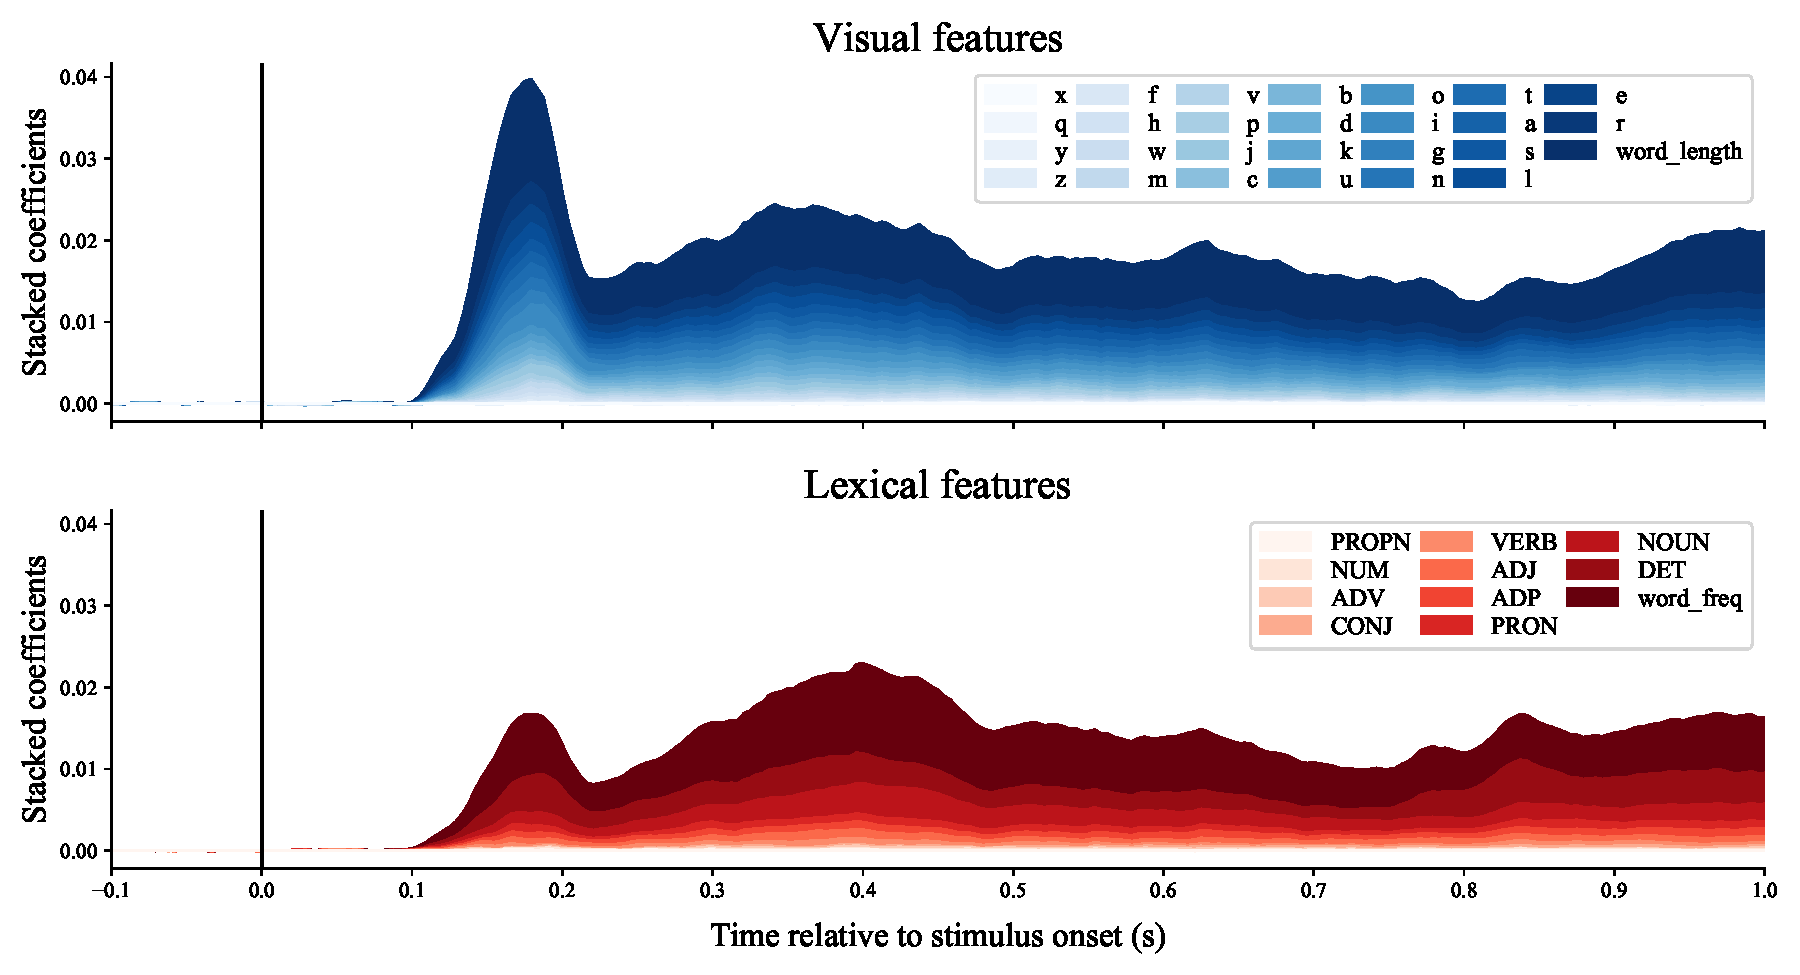
\includegraphics[width=\textwidth, trim=0cm 0cm 0cm 0cm, clip=True]{figures/meg_result.pdf}
  \caption{Cumulative estimates of word features as a function of time relative to word onset (chance level = 0). The dark blue area (word length) and dark red area (word frequency) correspond to the same data as those of the B2B average across subjects presented in \ref{fig:meg_twocurves}. A variety of visual features peak around 150ms, while a variety of lexical features tend to peak around 400ms.}
  \label{fig:megresult}
\end{figure}
